\XtoCBlock{Sequencer}
\label{block:Sequencer}
\begin{figure}[H]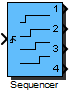
\includegraphics{Sequencer}\end{figure} 

\begin{XtoCtabular}{Inports}
Start & Start signal. Rising flank triggers sequence\tabularnewline
\hline
\end{XtoCtabular}


\begin{XtoCtabular}{Outports}
Out1 & Output \#1\tabularnewline
\hline
Out2 & Output \#2\tabularnewline
\hline
Out3 & Output \#3\tabularnewline
\hline
Out4 & Output \#4\tabularnewline
\hline
\end{XtoCtabular}

\begin{XtoCtabular}{Mask Parameters}
Delay1 & Time delay for output 1\tabularnewline
\hline
Delay2 & Time delay for output 2\tabularnewline
\hline
Delay3 & Time delay for output 3\tabularnewline
\hline
Delay4 & Time delay for output 4\tabularnewline
\hline
ts\_fact & Multiplication factor of base sampling time (in integer format)\tabularnewline
\hline
\end{XtoCtabular}

\subsubsection*{Description:}
Generation of time delayed (enable) sequence.

% include optional documentation file
\InputIfFileExists{\XcHomePath/Library/General/Doc/Sequencer_Info.tex}{\vspace{1ex}}{}

\subsubsection*{Implementations:}
\begin{tabular}{l l}
\textbf{FiP8} & 8 Bit Fixed Point Implementation\tabularnewline
\textbf{FiP16} & 16 Bit Fixed Point Implementation\tabularnewline
\textbf{FiP32} & 32 Bit Fixed Point Implementation\tabularnewline
\textbf{Float32} & 32 Bit Floating Point Implementation\tabularnewline
\textbf{Float64} & 64 Bit Floating Point Implementation\tabularnewline
\end{tabular}

\XtoCImplementation{FiP8}
\index{Block ID!448}
\nopagebreak[0]
% Implementation details
\begin{tabular}{l l}
\textbf{Name} & FiP8 \tabularnewline
\textbf{ID} & 448 \tabularnewline
\textbf{Revision} & 1.0 \tabularnewline
\textbf{C filename} & Sequencer\_FiP8.c \tabularnewline
\textbf{H filename} & Sequencer\_FiP8.h \tabularnewline
\end{tabular}
\vspace{1ex}

8 Bit Fixed Point Implementation

\begin{XtoCtabular}{Controller Parameters}
delay1 & Time delay for output 1\tabularnewline
\hline
delay2 & Time delay for output 2\tabularnewline
\hline
delay3 & Time delay for output 3\tabularnewline
\hline
delay4 & Time delay for output 4\tabularnewline
\hline
cnt & Timer value\tabularnewline
\hline
start\_old & Start value from previous cycle\tabularnewline
\hline
\end{XtoCtabular}

% Implementation data structure
\XtoCDataStruct{Data Structure:}
\begin{lstlisting}
typedef struct {
     uint16        ID;
     int8          *Start;
     int8          Out1;
     int8          Out2;
     int8          Out3;
     int8          Out4;
     uint16        delay1;
     uint16        delay2;
     uint16        delay3;
     uint16        delay4;
     uint16        cnt;
     int8          start_old;
} SEQUENCER_FIP8;
\end{lstlisting}

\ifdefined \AddTestReports
\InputIfFileExists{\XcHomePath/Library/General/Doc/Test_Sequencer_FiP8.tex}{}{}
\fi
\XtoCImplementation{FiP16}
\index{Block ID!449}
\nopagebreak[0]
% Implementation details
\begin{tabular}{l l}
\textbf{Name} & FiP16 \tabularnewline
\textbf{ID} & 449 \tabularnewline
\textbf{Revision} & 1.0 \tabularnewline
\textbf{C filename} & Sequencer\_FiP16.c \tabularnewline
\textbf{H filename} & Sequencer\_FiP16.h \tabularnewline
\end{tabular}
\vspace{1ex}

16 Bit Fixed Point Implementation

\begin{XtoCtabular}{Controller Parameters}
delay1 & Time delay for output 1\tabularnewline
\hline
delay2 & Time delay for output 2\tabularnewline
\hline
delay3 & Time delay for output 3\tabularnewline
\hline
delay4 & Time delay for output 4\tabularnewline
\hline
cnt & Timer value\tabularnewline
\hline
start\_old & Start value from previous cycle\tabularnewline
\hline
\end{XtoCtabular}

% Implementation data structure
\XtoCDataStruct{Data Structure:}
\begin{lstlisting}
typedef struct {
     uint16        ID;
     int16         *Start;
     int16         Out1;
     int16         Out2;
     int16         Out3;
     int16         Out4;
     uint16        delay1;
     uint16        delay2;
     uint16        delay3;
     uint16        delay4;
     uint16        cnt;
     int16         start_old;
} SEQUENCER_FIP16;
\end{lstlisting}

\ifdefined \AddTestReports
\InputIfFileExists{\XcHomePath/Library/General/Doc/Test_Sequencer_FiP16.tex}{}{}
\fi
\XtoCImplementation{FiP32}
\index{Block ID!450}
\nopagebreak[0]
% Implementation details
\begin{tabular}{l l}
\textbf{Name} & FiP32 \tabularnewline
\textbf{ID} & 450 \tabularnewline
\textbf{Revision} & 1.0 \tabularnewline
\textbf{C filename} & Sequencer\_FiP32.c \tabularnewline
\textbf{H filename} & Sequencer\_FiP32.h \tabularnewline
\end{tabular}
\vspace{1ex}

32 Bit Fixed Point Implementation

\begin{XtoCtabular}{Controller Parameters}
delay1 & Time delay for output 1\tabularnewline
\hline
delay2 & Time delay for output 2\tabularnewline
\hline
delay3 & Time delay for output 3\tabularnewline
\hline
delay4 & Time delay for output 4\tabularnewline
\hline
cnt & Timer value\tabularnewline
\hline
start\_old & Start value from previous cycle\tabularnewline
\hline
\end{XtoCtabular}

% Implementation data structure
\XtoCDataStruct{Data Structure:}
\begin{lstlisting}
typedef struct {
     uint16        ID;
     int32         *Start;
     int32         Out1;
     int32         Out2;
     int32         Out3;
     int32         Out4;
     uint16        delay1;
     uint16        delay2;
     uint16        delay3;
     uint16        delay4;
     uint16        cnt;
     int32         start_old;
} SEQUENCER_FIP32;
\end{lstlisting}

\ifdefined \AddTestReports
\InputIfFileExists{\XcHomePath/Library/General/Doc/Test_Sequencer_FiP32.tex}{}{}
\fi
\XtoCImplementation{Float32}
\index{Block ID!451}
\nopagebreak[0]
% Implementation details
\begin{tabular}{l l}
\textbf{Name} & Float32 \tabularnewline
\textbf{ID} & 451 \tabularnewline
\textbf{Revision} & 0.1 \tabularnewline
\textbf{C filename} & Sequencer\_Float32.c \tabularnewline
\textbf{H filename} & Sequencer\_Float32.h \tabularnewline
\end{tabular}
\vspace{1ex}

32 Bit Floating Point Implementation

\begin{XtoCtabular}{Controller Parameters}
delay1 & Time delay for output 1\tabularnewline
\hline
delay2 & Time delay for output 2\tabularnewline
\hline
delay3 & Time delay for output 3\tabularnewline
\hline
delay4 & Time delay for output 4\tabularnewline
\hline
cnt & Timer value\tabularnewline
\hline
start\_old & Start value from previous cycle\tabularnewline
\hline
\end{XtoCtabular}

% Implementation data structure
\XtoCDataStruct{Data Structure:}
\begin{lstlisting}
typedef struct {
     uint16        ID;
     float32       *Start;
     float32       Out1;
     float32       Out2;
     float32       Out3;
     float32       Out4;
     uint16        delay1;
     uint16        delay2;
     uint16        delay3;
     uint16        delay4;
     uint16        cnt;
     float32       start_old;
} SEQUENCER_FLOAT32;
\end{lstlisting}

\ifdefined \AddTestReports
\InputIfFileExists{\XcHomePath/Library/General/Doc/Test_Sequencer_Float32.tex}{}{}
\fi
\XtoCImplementation{Float64}
\index{Block ID!452}
\nopagebreak[0]
% Implementation details
\begin{tabular}{l l}
\textbf{Name} & Float64 \tabularnewline
\textbf{ID} & 452 \tabularnewline
\textbf{Revision} & 0.1 \tabularnewline
\textbf{C filename} & Sequencer\_Float64.c \tabularnewline
\textbf{H filename} & Sequencer\_Float64.h \tabularnewline
\end{tabular}
\vspace{1ex}

64 Bit Floating Point Implementation

\begin{XtoCtabular}{Controller Parameters}
delay1 & Time delay for output 1\tabularnewline
\hline
delay2 & Time delay for output 2\tabularnewline
\hline
delay3 & Time delay for output 3\tabularnewline
\hline
delay4 & Time delay for output 4\tabularnewline
\hline
cnt & Timer value\tabularnewline
\hline
start\_old & Start value from previous cycle\tabularnewline
\hline
\end{XtoCtabular}

% Implementation data structure
\XtoCDataStruct{Data Structure:}
\begin{lstlisting}
typedef struct {
     uint16        ID;
     float64       *Start;
     float64       Out1;
     float64       Out2;
     float64       Out3;
     float64       Out4;
     uint16        delay1;
     uint16        delay2;
     uint16        delay3;
     uint16        delay4;
     uint16        cnt;
     float64       start_old;
} SEQUENCER_FLOAT64;
\end{lstlisting}

\ifdefined \AddTestReports
\InputIfFileExists{\XcHomePath/Library/General/Doc/Test_Sequencer_Float64.tex}{}{}
\fi
